
\documentclass[10pt,a4paper]{article}
\usepackage[utf8]{inputenc}
\usepackage{amsmath}
\usepackage{amsfonts}
\usepackage{amssymb}
\usepackage{graphicx}
\author{Marcelo Lynch}
\usepackage[margin=2.5in]{geometry}


\newcommand{\N}{\mathbb{N}}
\newcommand{\Z}{\mathbb{Z}}
\newcommand{\Q}{\mathbb{Q}}
\newcommand{\R}{\mathbb{R}}
\newcommand{\C}{\mathbb{C}}
\newcommand{\Rr}{\mathcal{R}}
\newcommand{\G}{\Gamma}
\newcommand{\ra}{\rightarrow}
\newcommand{\bra}{\textcolor{blue}{\longrightarrow}}
\newcommand{\bla}{\textcolor{blue}{\longleftarrow}}
\newcommand{\rra}{\textcolor{red}{\longrightarrow}}
\newcommand{\rla}{\textcolor{red}{\longleftarrow}}
\newcommand{\Ra}{\Rightarrow}
\renewcommand{\S}{\Sigma}
\newcommand{\bz}{\bm{0}}
\newcommand{\bo}{\bm{1}}

\newcommand{\peq}{\preceq}

\renewcommand{\a}{\alpha}
\renewcommand{\b}{\beta}
\newcommand{\g}{\gamma}

\renewcommand{\L}{\mathcal{L}}
\newcommand{\I}{\mathcal{I}}
\newcommand{\genericfol}{\L = (\mathcal{F})}
\newcommand{\U}{\mathcal{U}}

\title{\vspace{-1.6cm}Visualizando $c^{\aleph_0} = (2^{\aleph_0})^{\aleph_0} = 2^{\aleph_0 \cdot \aleph_0} = 2^{\aleph_0} = c$ }
\author{Marcelo Lynch}
\date{}
\begin{document}

\maketitle


Supongamos una lista infinita de números del intervalo $(0,1)$: $a_0, a_1, a_2, \cdots$. Podemos escribirlos desarrollando la expansión decimal, uno abajo del otro:

\[ 0,a_0^0\ a_0^1\ a_0^2\ a_0^3\ a_0^4\ \cdots \]
\[ 0,a_1^0\ a_1^1\ a_1^2\ a_1^3\ a_1^4\ \cdots \]
\[ 0,a_2^0\ a_2^1\ a_2^2\ a_2^3\ a_2^4\ \cdots \]
\[ 0,a_3^0\ a_3^1\ a_3^2\ a_3^3\ a_3^4\ \cdots \]
\[ 0,a_4^0\ a_4^1\ a_4^2\ a_4^3\ a_4^4\ \cdots \]
\[\ \ \vdots\ \hspace{30px}  \hspace{30px} \]
Donde $a_i^j$ es el $j$-ésimo dígito (despues de la coma) del numero $a_i$\\\

Estos números siempre se van a poder escribir como ``cero coma algo'', porque están en $(0,1)$, entonces podemos ahorrarnos escribir eso y solamente identificar a cada numero con los digitos que vienen después de la coma:
 
\[ a_0^0\ \ a_0^1\ \ a_0^2\ \ a_0^3\ \ a_0^4\ \ \cdots \]
\[ a_1^0\ \ a_1^1\ \ a_1^2\ \ a_1^3\ \ a_1^4\ \ \cdots \]
\[ a_2^0\ \ a_2^1\ \ a_2^2\ \ a_2^3\ \ a_2^4\ \ \cdots \]
\[ a_3^0\ \ a_3^1\ \ a_3^2\ \ a_3^3\ \ a_3^4\ \ \cdots \]
\[ a_4^0\ \ a_4^1\ \ a_4^2\ \ a_4^3\ \ a_4^4\ \  \cdots \]
\[\ \ \ \ \ \ \hspace{50px} \vdots\ \ \vdots\ \ \vdots \hspace{50px} \]

¿Cómo hacemos para transformar esto en un único número? El truco está en recorrer esta ``grilla infinita'' de manera tal de no perdernos ningun dígito, y armar los dígitos después de la coma de nuestro nuevo número:

\begin{figure}[h!]
\centering
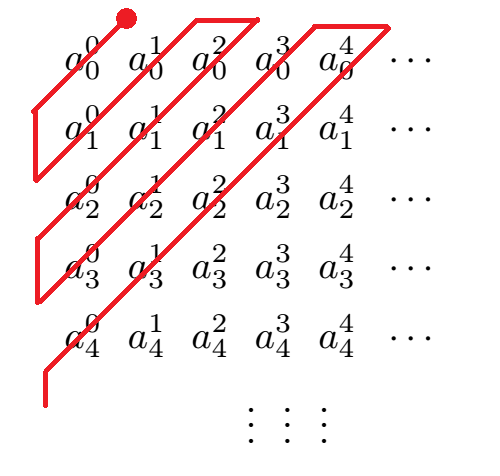
\includegraphics[scale=0.6]{diago2.png}
\end{figure}

Haciendo este zigzag podemos ir \textbf{recorriendo todos los dígitos sin saltearnos ninguno}. Con este recorrido podemos armar \textbf{un único número real}: 

\[ x = 0,a_0^0\ a_1^0\ a_0^1 \ a_0^2\ a_1^1\ a_2^0 \ \cdots \]

Y así  \textbf{los infinitos números quedan condensados en uno solo}. Notemos que dado este número podemos reconstruir la tabla, si la arrancamos vacía y vamos llenando los espacios mientras recorremos con el mismo zig-zag, es decir, \textbf{no se pierde información}.

\end{document}